%*******10********20********30********40********50********60********70********80

\chap{Simulation of Mechanical Properties Of ASR and DEF Expanded Concrete}

\section{General}

In this chapter, three-dimensional expanded concrete models are tested under uni-axial compression condition, and the mechanical properties obtained from simulation are compared with previous experimental results from other researchers.

The purpose of this study is for the prediction of the behavior and residual capacity of ASR or DEF expanded concrete, especially in uni-axial compression.


\clearpage
\section{Uni-axial compression result for $10 \times 10 \times 10$ mm Expanded Models}

%*******10********20********30********40********50********60********70********80
\subsection{Uni-axial compression result for $10 \times 10 \times 10$ mm ASR Expanded Models}

In this section, simulation uni-axial compression test on a single aggregate case in size only $10 \times 10 \times 10$ mm is presented, as shown in Figure \ref{sdfsdfasr}. Displacement of loading boundary is controlled in this analysis. In each step of loading, the top boundary of the concrete model moves downwards 0.002 mm.

It is easier to analyze the behavior under loading condition in very small scale around coarse aggregate in a relatively smaller model.

The model is expanded by ASR following the process in chapter 2 and 3. 0.001 initial strain is introduced in each step at the interfaces between the aggregate and paste elements. Totally 20 steps of expansion are done.

%TODO: Single Aggregate 3D, 2D

\begin{figure}[h!]
\centering
%*******
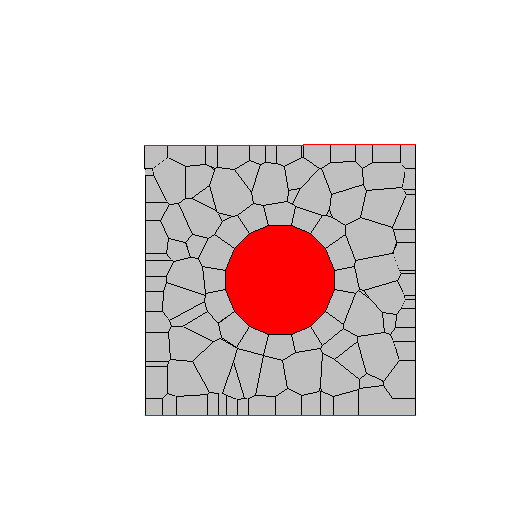
\includegraphics[width=0.4\linewidth]{Files/Small_ASR/CR/DEP5-STEP(001).png}
\caption{Single Aggregate Case in Size $10 \times 10 \times 10$ mm}
\label{sdfsdfasr}
\end{figure}

\begin{figure}[ht!]
\centering

    %*******
    \begin{subfigure}{.33\textwidth}
      \centering
      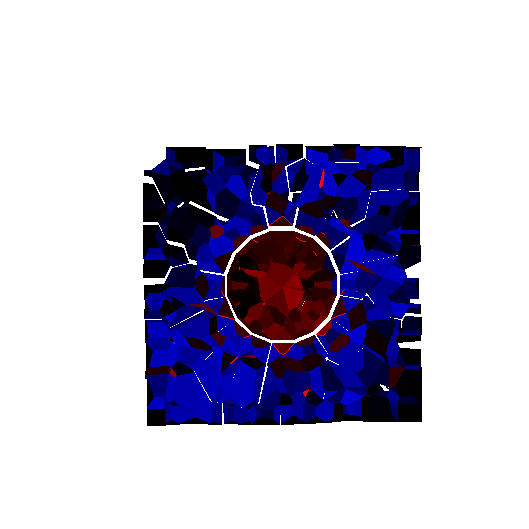
\includegraphics[width=1.0\linewidth]{Files/Small_ASR/IS2/DEP5-STEP(020).png}
      \caption{Before Loading}
    \end{subfigure}%
    \begin{subfigure}{.33\textwidth}
      \centering
      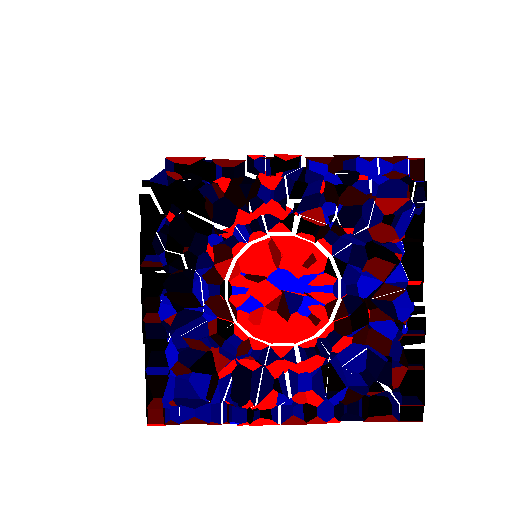
\includegraphics[width=1.0\linewidth]{Files/Small_ASR/IS2/DEP5-STEP(040).png}
      \caption{Loading Step 20}
      \end{subfigure}%
      %*******
      \begin{subfigure}{.33\textwidth}
        \centering
        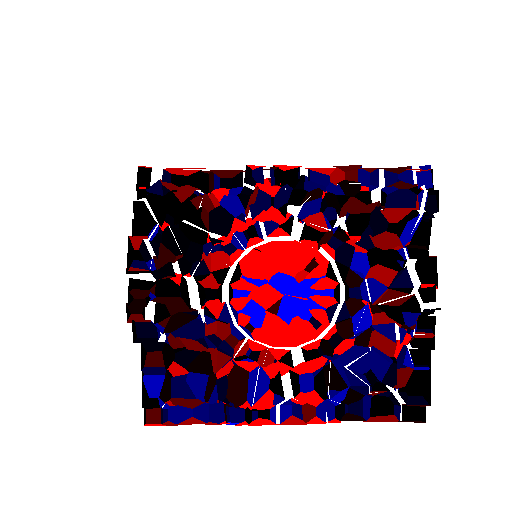
\includegraphics[width=1.0\linewidth]{Files/Small_ASR/IS2/DEP5-STEP(060).png}
        \caption{Loading Step 40}
      \end{subfigure}
      %*******

    %*******
    \begin{subfigure}{.33\textwidth}
      \centering
      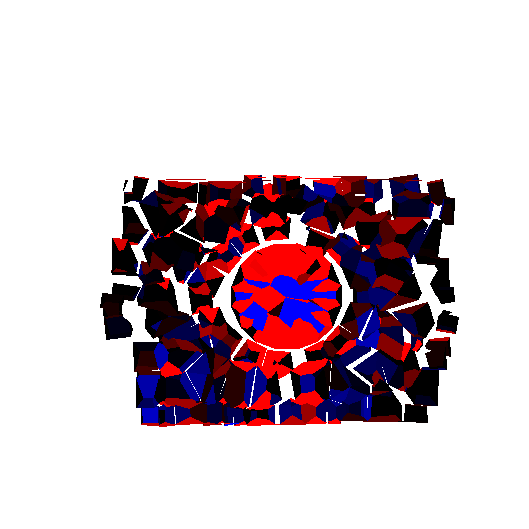
\includegraphics[width=1.0\linewidth]{Files/Small_ASR/IS2/DEP5-STEP(080).png}
      \caption{Loading Step 60}
    \end{subfigure}%
    \begin{subfigure}{.33\textwidth}
      \centering
      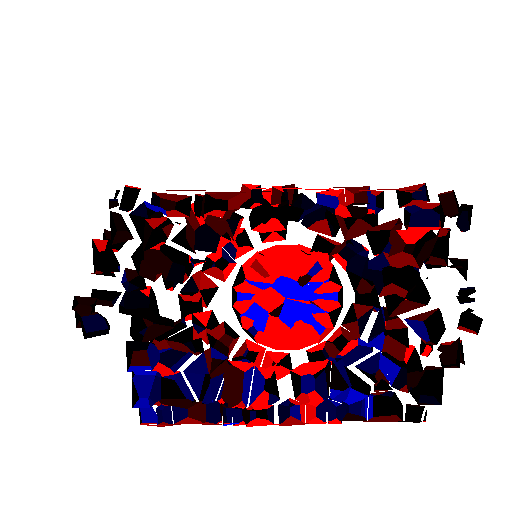
\includegraphics[width=1.0\linewidth]{Files/Small_ASR/IS2/DEP5-STEP(100).png}
      \caption{Loading Step 80}
      \end{subfigure}%
      %*******
      \begin{subfigure}{.33\textwidth}
        \centering
        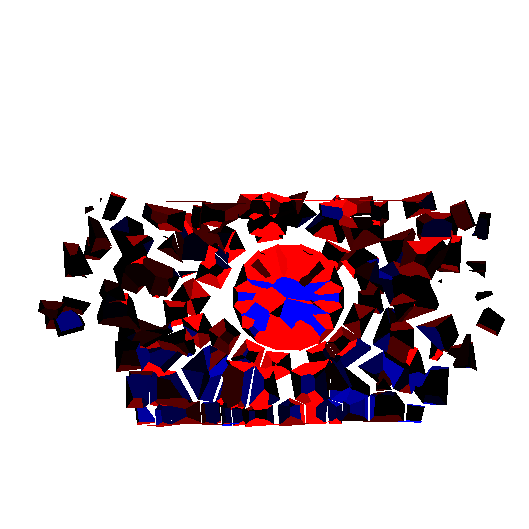
\includegraphics[width=1.0\linewidth]{Files/Small_ASR/IS2/DEP5-STEP(120).png}
        \caption{Loading Step 100}
      \end{subfigure}
      %*******
  \begin{subfigure}{0.8\textwidth}
  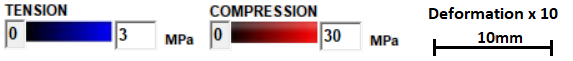
\includegraphics[width=0.8\linewidth]{Files/exp_3D/tagCS30s.png}
\end{subfigure}%

  \caption{ASR Loading for $10 \times 10 \times 10$ mm model, Fixed Boundary Condition}
  \label{fig:ASR_Loading_s_fix}
\end{figure}

For Loading with fixed boundary condition, Figure \ref{fig:ASR_Loading_s_fix} here shows the initial stress condition during loading in loading step 0, 20, 30, 60 and 80.

With increasing the step of loading, in each step the top surface moves downwards for 0.002 mm. Compressive strength generate together with the deformation, especially concentrated horizontally in the middle of the model.

As the top and bottom boundary are horizontally, elements in the middle of model start to move away from the center of model firstly, followed by the failure of whole model.

If we compare its behavior with free boundary condition loading, shown in Figure \ref{fig:ASR_Loading_s_free}, it can be seen that the way crack generate and deformation generate is totally different in these two cases.

In Free boundary loading, the cracks are more easier to open without the restrain from top and bottom boundary. The deformation in horizontal direction is more uniformed. Inner Stress distributed more uniformly in the free boundary loading case.

\begin{figure}[ht!]
\centering

    %*******
    \begin{subfigure}{.33\textwidth}
      \centering
      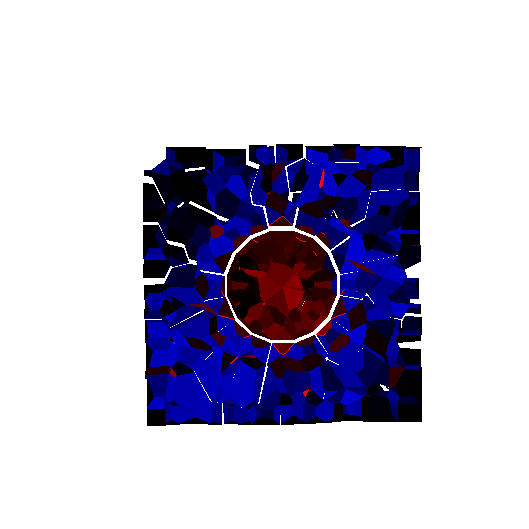
\includegraphics[width=1.0\linewidth]{Files/Small_ASR/IS2/DEP5-STEP(020).png}
      \caption{Before Loading}
    \end{subfigure}%
    \begin{subfigure}{.33\textwidth}
      \centering
      \includegraphics[width=1.0\linewidth]{Files/Small_ASR/Free_IS2/DEP5-STEP(040).png}
      \caption{Loading Step 20}
      \end{subfigure}%
      %*******
      \begin{subfigure}{.33\textwidth}
        \centering
        \includegraphics[width=1.0\linewidth]{Files/Small_ASR/Free_IS2/DEP5-STEP(060).png}
        \caption{Loading Step 40}
      \end{subfigure}
      %*******

    %*******
    \begin{subfigure}{.33\textwidth}
      \centering
      \includegraphics[width=1.0\linewidth]{Files/Small_ASR/Free_IS2/DEP5-STEP(080).png}
      \caption{Loading Step 60}
    \end{subfigure}%
    \begin{subfigure}{.33\textwidth}
      \centering
      \includegraphics[width=1.0\linewidth]{Files/Small_ASR/Free_IS2/DEP5-STEP(100).png}
      \caption{Loading Step 80}
      \end{subfigure}%
      %*******
      \begin{subfigure}{.33\textwidth}
        \centering
        \includegraphics[width=1.0\linewidth]{Files/Small_ASR/Free_IS2/DEP5-STEP(120).png}
        \caption{Loading Step 100}
      \end{subfigure}
      %*******
  \begin{subfigure}{0.8\textwidth}
  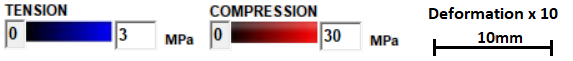
\includegraphics[width=0.8\linewidth]{Files/exp_3D/tagCS30s.png}
\end{subfigure}%

  \caption{ASR Loading for $10 \times 10 \times 10$ mm model, Free Boundary Condition}
  \label{fig:ASR_Loading_s_free}
\end{figure}

From the small size model it can be confirmed the workability of uni-axial compression test on a single aggregate $10 \times 10 \times 10$ mm model. Later, uni-axial compression test on full size model($100 \times 100 \times 100$ mm) damaged by ASR expansion will be carried out.

\clearpage
%*******10********20********30********40********50********60********70********80
\subsection{Uni-axial compression result for $10 \times 10 \times 10$ mm DEF Expanded Models}

Simulation of uni-axial compression test on a single aggregate case in size $10 \times 10 \times 10$ mm is presented also for DEF damaged concrete model (Figure \ref{cdefsma}). Same as in ASR case, in each step of loading, the top boundary of the concrete model moves downwards 0.002 mm.

The model is expanded by DEF following the process in chapter 2 and 3. 0.0003 initial strain is given to all paste interfaces uniformly in this simulation. Totally 20 steps of expansion are done.

%TODO: Single Aggregate 3D, 2D

\begin{figure}[h!]
\centering
%*******
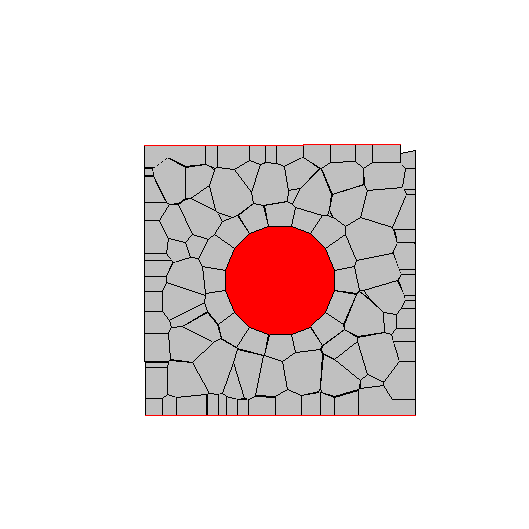
\includegraphics[width=0.4\linewidth]{Files/Small_DEF/CR/DEP5-STEP(001).png}
\caption{Single Aggregate Case in Size $10 \times 10 \times 10$ mm}
\label{cdefsma}
\end{figure}

\begin{figure}[ht!]
\centering

    %*******
    \begin{subfigure}{.33\textwidth}
      \centering
      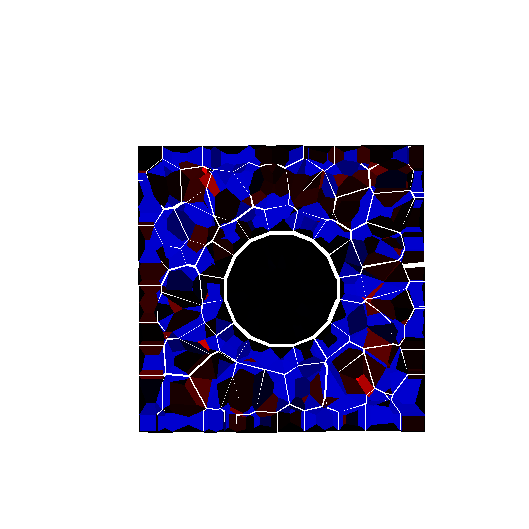
\includegraphics[width=1.0\linewidth]{Files/Small_DEF/IS2/DEP5-STEP(020).png}
      \caption{Before Loading}
    \end{subfigure}%
    \begin{subfigure}{.33\textwidth}
      \centering
      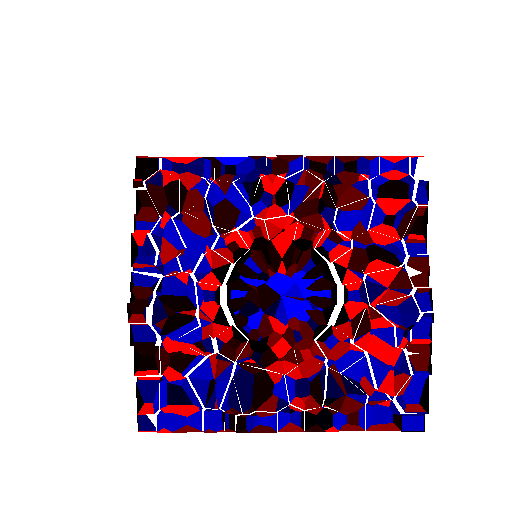
\includegraphics[width=1.0\linewidth]{Files/Small_DEF/IS2/DEP5-STEP(040).png}
      \caption{Loading Step 20}
      \end{subfigure}%
      %*******
      \begin{subfigure}{.33\textwidth}
        \centering
        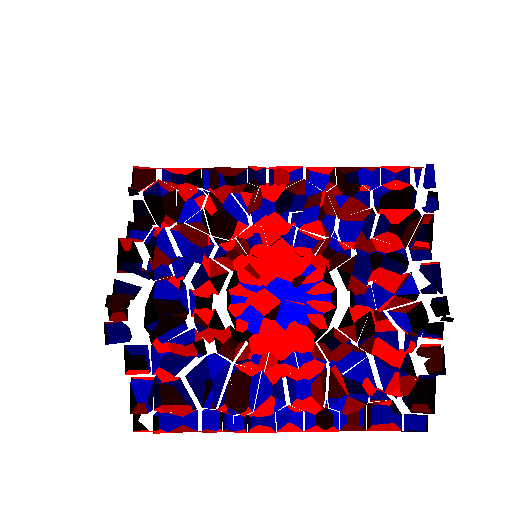
\includegraphics[width=1.0\linewidth]{Files/Small_DEF/IS2/DEP5-STEP(060).png}
        \caption{Loading Step 40}
      \end{subfigure}
      %*******

    %*******
    \begin{subfigure}{.33\textwidth}
      \centering
      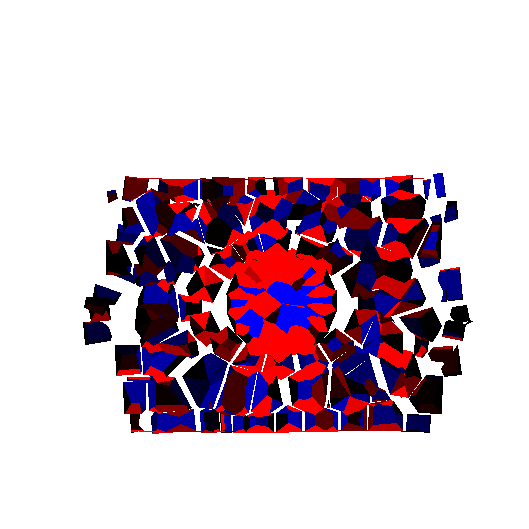
\includegraphics[width=1.0\linewidth]{Files/Small_DEF/IS2/DEP5-STEP(080).png}
      \caption{Loading Step 60}
    \end{subfigure}%
    \begin{subfigure}{.33\textwidth}
      \centering
      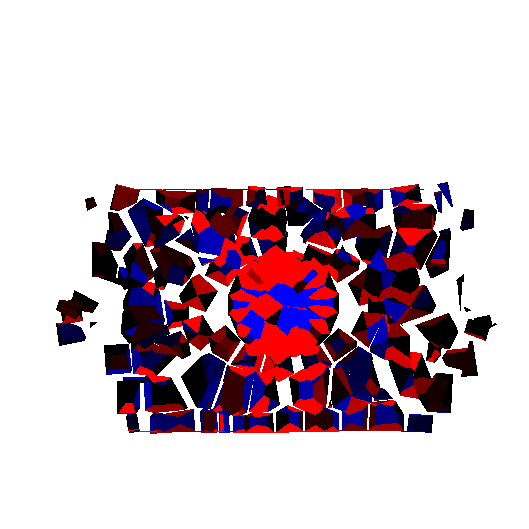
\includegraphics[width=1.0\linewidth]{Files/Small_DEF/IS2/DEP5-STEP(100).png}
      \caption{Loading Step 80}
      \end{subfigure}%
      %*******
      \begin{subfigure}{.33\textwidth}
        \centering
        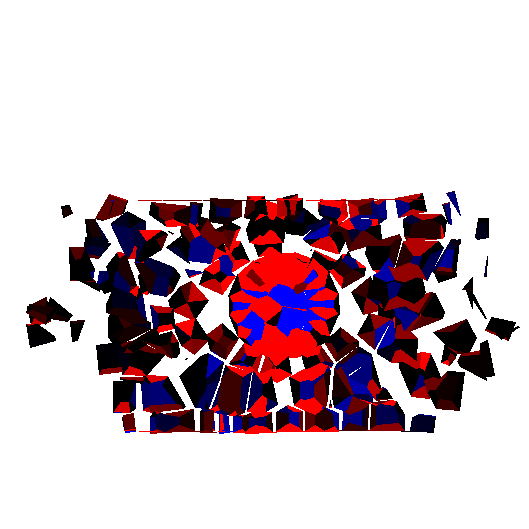
\includegraphics[width=1.0\linewidth]{Files/Small_DEF/IS2/DEP5-STEP(120).png}
        \caption{Loading Step 100}
      \end{subfigure}
      %*******
  \begin{subfigure}{0.8\textwidth}
  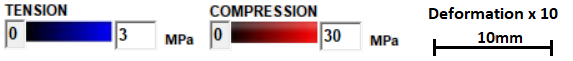
\includegraphics[width=0.8\linewidth]{Files/exp_3D/tagCS30s.png}
\end{subfigure}%

  \caption{DEF Loading for $10 \times 10 \times 10$ mm model, Fixed Boundary Condition}
  \label{fig:DEF_Loading_s_fix}
\end{figure}

For Loading with fixed boundary condition, Figure \ref{fig:DEF_Loading_s_fix} here shows the initial stress condition during loading in loading step 0, 20, 30, 60 and 80.

With increasing the step of loading, in each step the top surface moves downwards for 0.002 mm. Compressive strength generate together with the deformation, especially concentrated horizontally in the middle of the model.

As the top and bottom boundary are horizontally, elements in the middle of model start to move away from the center of model firstly, followed by the failure of whole model.

If we compare its behavior with free boundary condition loading, shown in Figure \ref{fig:DEF_Loading_s_free}, it can be seen that the way crack generate and deformation generate is totally different in these two cases.

In Free boundary loading, the cracks are more easier to open without the restrain from top and bottom boundary. The deformation in horizontal direction is more uniformed. Inner Stress distributed more uniformly in the free boundary loading case.

\begin{figure}[ht!]
\centering

    %*******
    \begin{subfigure}{.33\textwidth}
      \centering
      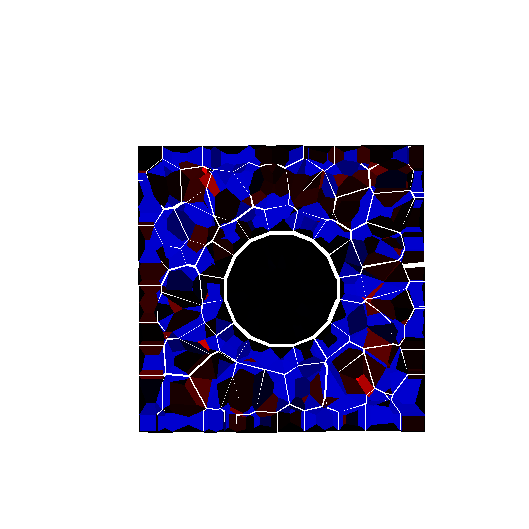
\includegraphics[width=1.0\linewidth]{Files/Small_DEF/IS2/DEP5-STEP(020).png}
      \caption{Before Loading}
    \end{subfigure}%
    \begin{subfigure}{.33\textwidth}
      \centering
      \includegraphics[width=1.0\linewidth]{Files/Small_DEF/Free_IS2/DEP5-STEP(040).png}
      \caption{Loading Step 20}
      \end{subfigure}%
      %*******
      \begin{subfigure}{.33\textwidth}
        \centering
        \includegraphics[width=1.0\linewidth]{Files/Small_DEF/Free_IS2/DEP5-STEP(060).png}
        \caption{Loading Step 40}
      \end{subfigure}
      %*******

    %*******
    \begin{subfigure}{.33\textwidth}
      \centering
      \includegraphics[width=1.0\linewidth]{Files/Small_DEF/Free_IS2/DEP5-STEP(080).png}
      \caption{Loading Step 60}
    \end{subfigure}%
    \begin{subfigure}{.33\textwidth}
      \centering
      \includegraphics[width=1.0\linewidth]{Files/Small_DEF/Free_IS2/DEP5-STEP(100).png}
      \caption{Loading Step 80}
      \end{subfigure}%
      %*******
      \begin{subfigure}{.33\textwidth}
        \centering
        \includegraphics[width=1.0\linewidth]{Files/Small_DEF/Free_IS2/DEP5-STEP(120).png}
        \caption{Loading Step 100}
      \end{subfigure}
      %*******
  \begin{subfigure}{0.8\textwidth}
  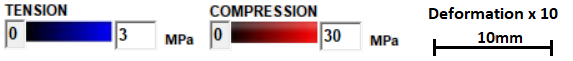
\includegraphics[width=0.8\linewidth]{Files/exp_3D/tagCS30s.png}
\end{subfigure}%

  \caption{DEF Loading for $10 \times 10 \times 10$ mm model, Free Boundary Condition}
  \label{fig:DEF_Loading_s_free}
\end{figure}

Later, uni-axial compression test on full size model($100 \times 100 \times 100$ mm) damaged by DEF expansion will also be carried out.


\clearpage

\section{Uni-axial compression result for $100 \times 100 \times 100$ mm Expanded Models}

Displacement of loading boundary is controlled in this analysis. In each step of loading, the top boundary of the concrete model moves downwards 0.02 mm.

\begin{figure}[ht!]
\centering
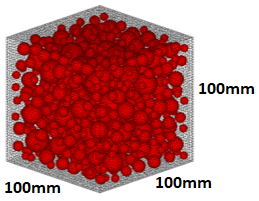
\includegraphics[width=.3\linewidth]{Files/Aggregate/A30.png}
  \caption{30\% Coarse Aggregate}
  \label{fig:A30_model}
\end{figure}

Figure \ref{fig:ASR_Loading} and Figure \ref{fig:DEF_Loading} here presented the internal stress condition of 2 example cases for ASR and DEF loading of Fixed boundary condition, seperately. In Figure , $100 \times 100 \times 100$ mm model with 30\% coarse aggregate is used, of which 75\% of all coarse aggregates are ASR reactived. While for DEF, same $100 \times 100 \times 100$ mm model with 30\% coarse aggregate is used, of which the center $75 \times 75 \times 75$ mm part has been given intensified DEF expansion, and gradually decrease until reaching the surface of the model.

It can be seen that with the increasing of vertical displacement applied to the expansion damaged models, compressive force generated in the concrete model,  and X shape cracking developed gradually until the failure of the structure is reached.

The internal stress reaction of ASR and DEF expanded concrete model is relatively close, but the maximum Compressive Strength and Elastic Modulus does show some of the differences.

And when considering free boundary condition loading, shown in Figure \ref{fig:ASR_Loading_free}, the top and bottom of the concrete model can move freely in horizontal directions, thus the X-shape cracking pattern shown in fix boundary loading cases does now show up here.

%A30P75FIX_3

\begin{figure}[ht]
\centering

    %*******
    \begin{subfigure}{.33\textwidth}
      \centering
      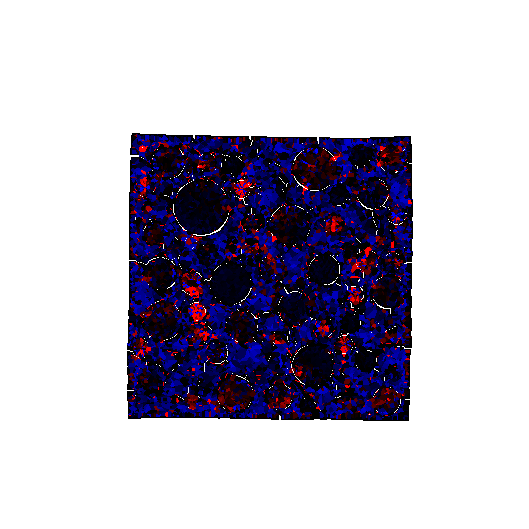
\includegraphics[width=1.0\linewidth]{Files/A30P75_3_IS/DEP50-STEP(020).png}
      \caption{Before Loading}
    \end{subfigure}%
    \begin{subfigure}{.33\textwidth}
      \centering
      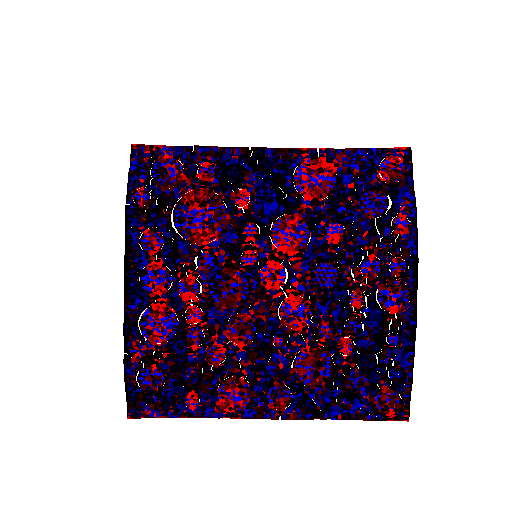
\includegraphics[width=1.0\linewidth]{Files/A30P75_3_IS/DEP50-STEP(040).png}
      \caption{Loading Step 20}
      \end{subfigure}%
      %*******
      \begin{subfigure}{.33\textwidth}
        \centering
        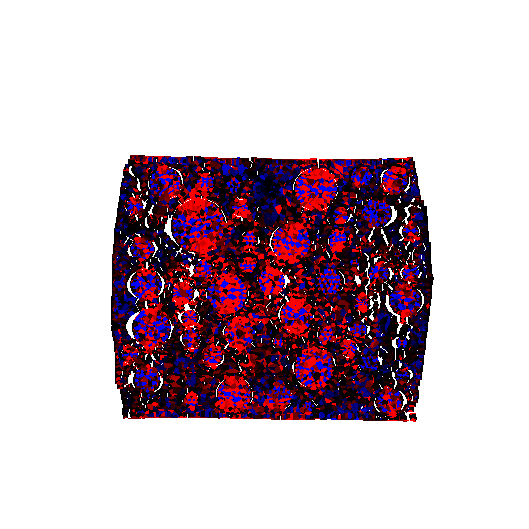
\includegraphics[width=1.0\linewidth]{Files/A30P75_3_IS/DEP50-STEP(060).png}
        \caption{Loading Step 40}
      \end{subfigure}
      %*******

    %*******
    \begin{subfigure}{.33\textwidth}
      \centering
      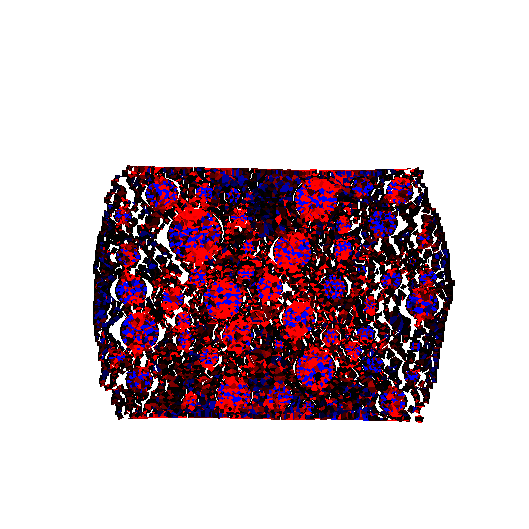
\includegraphics[width=1.0\linewidth]{Files/A30P75_3_IS/DEP50-STEP(080).png}
      \caption{Loading Step 60}
    \end{subfigure}%
    \begin{subfigure}{.33\textwidth}
      \centering
      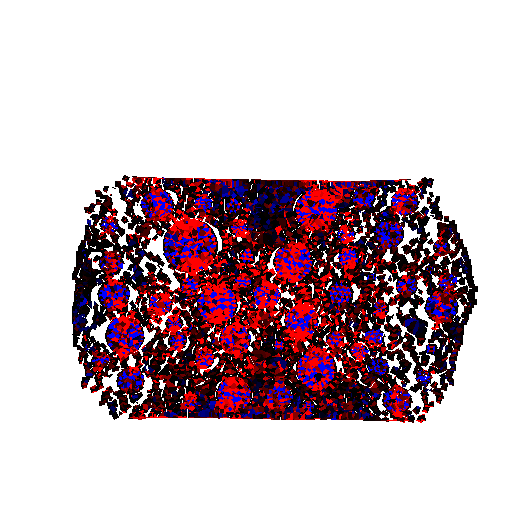
\includegraphics[width=1.0\linewidth]{Files/A30P75_3_IS/DEP50-STEP(100).png}
      \caption{Loading Step 80}
      \end{subfigure}%
      %*******
      \begin{subfigure}{.33\textwidth}
        \centering
        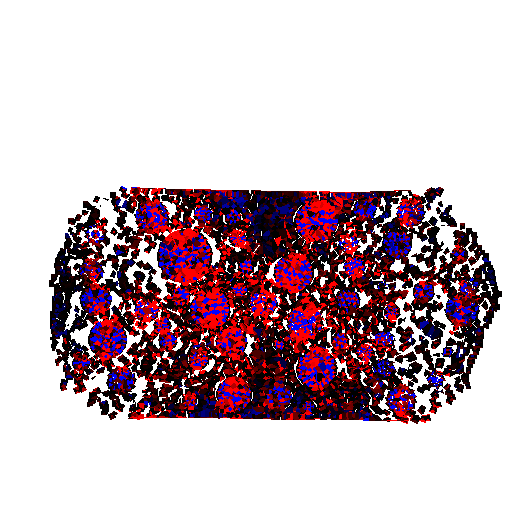
\includegraphics[width=1.0\linewidth]{Files/A30P75_3_IS/DEP50-STEP(120).png}
        \caption{Loading Step 100}
      \end{subfigure}
      %*******
  \begin{subfigure}{0.8\textwidth}
  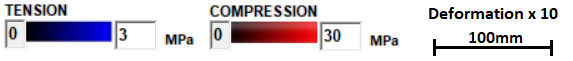
\includegraphics[width=0.8\linewidth]{Files/exp_3D/tagCS30.png}
\end{subfigure}%

  \caption{ASR Loading in Fixed Boundary Condition}
  \label{fig:ASR_Loading}
\end{figure}

\begin{figure}[ht]
\centering

    %*******
    \begin{subfigure}{.33\textwidth}
      \centering
      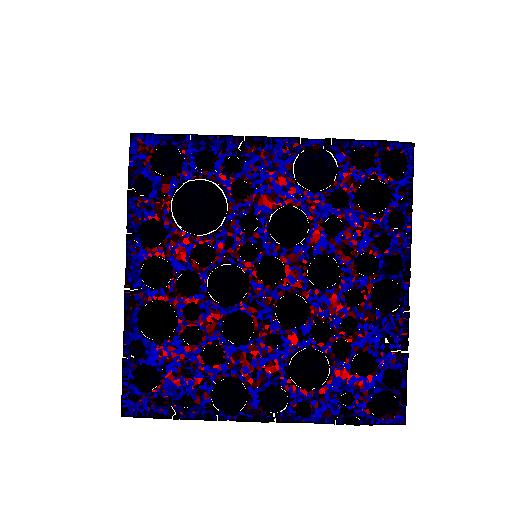
\includegraphics[width=1.0\linewidth]{Files/A30X-5C_3_IS/DEP50-STEP(020).png}
      \caption{Before Loading}
    \end{subfigure}%
    %*******
    \begin{subfigure}{.33\textwidth}
      \centering
      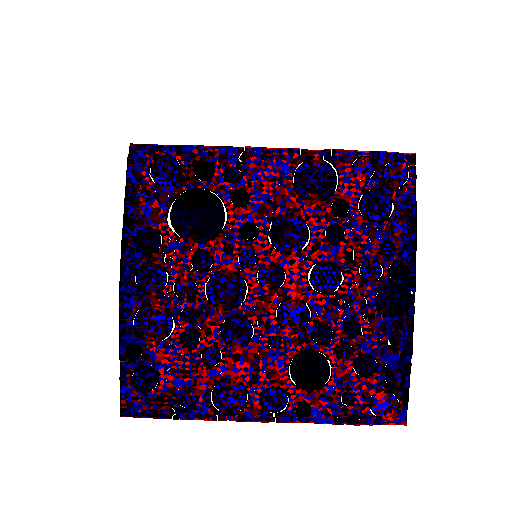
\includegraphics[width=1.0\linewidth]{Files/A30X-5C_3_IS/DEP50-STEP(040).png}
      \caption{Loading Step 20}
      \end{subfigure}%
      %*******
      \begin{subfigure}{.33\textwidth}
        \centering
        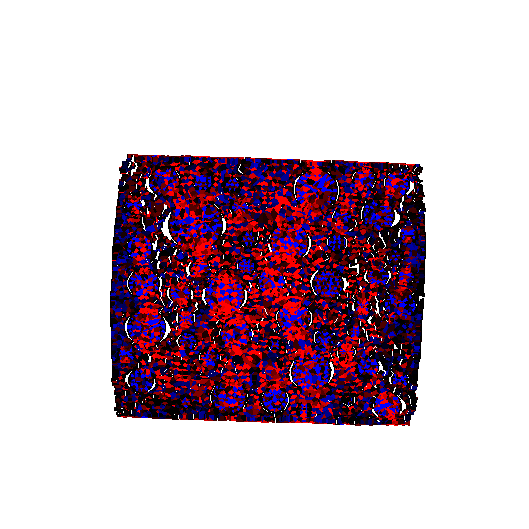
\includegraphics[width=1.0\linewidth]{Files/A30X-5C_3_IS/DEP50-STEP(060).png}
        \caption{Loading Step 40}
      \end{subfigure}
      %*******

    %*******
    \begin{subfigure}{.33\textwidth}
      \centering
      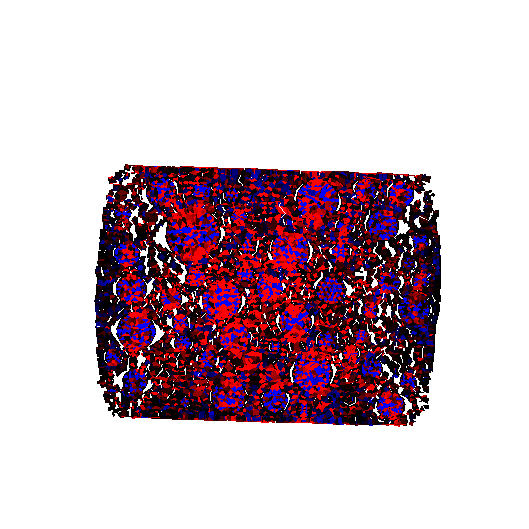
\includegraphics[width=1.0\linewidth]{Files/A30X-5C_3_IS/DEP50-STEP(080).png}
      \caption{Loading Step 60}
    \end{subfigure}%
    %*******
    \begin{subfigure}{.33\textwidth}
      \centering
      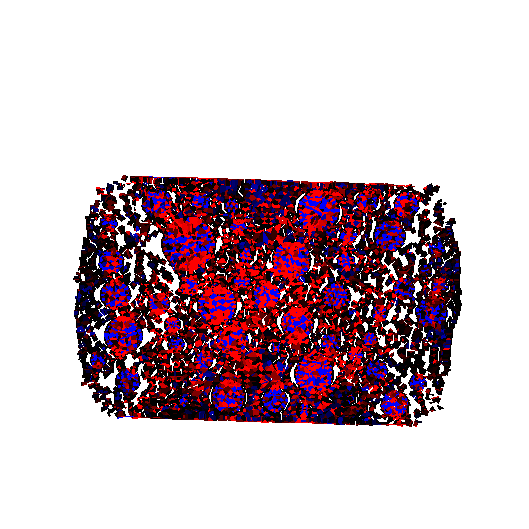
\includegraphics[width=1.0\linewidth]{Files/A30X-5C_3_IS/DEP50-STEP(100).png}
      \caption{Loading Step 80}
    \end{subfigure}%
    %*******
    \begin{subfigure}{.33\textwidth}
      \centering
      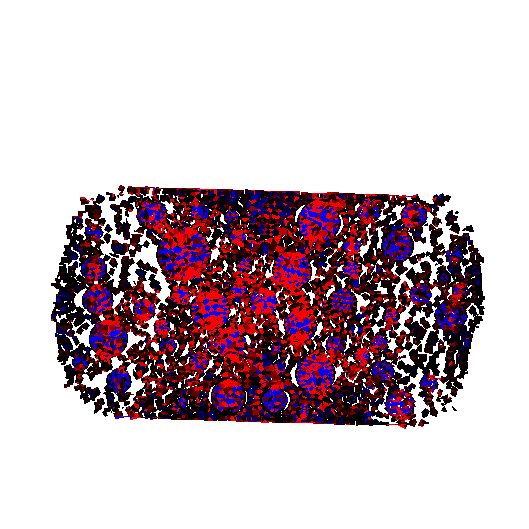
\includegraphics[width=1.0\linewidth]{Files/A30X-5C_3_IS/DEP50-STEP(120).png}
      \caption{Loading Step 100}
    \end{subfigure}
    %*******

    \begin{subfigure}{0.8\textwidth}
  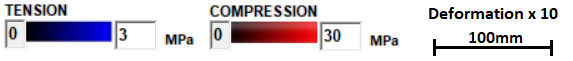
\includegraphics[width=0.8\linewidth]{Files/exp_3D/tagCS30.png}
\end{subfigure}%


  \caption{DEF Loading in Fixed Boundary Condition}
  \label{fig:DEF_Loading}
\end{figure}

%A30P75FIX_3

\begin{figure}[ht]
\centering

    %*******
    \begin{subfigure}{.33\textwidth}
      \centering
      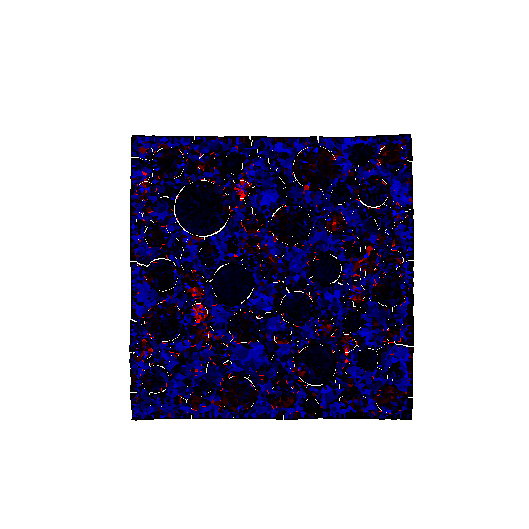
\includegraphics[width=1.0\linewidth]{Files/A30P75_3_IS_Free/DEP50-STEP(020).png}
      \caption{Before Loading}
    \end{subfigure}%
    \begin{subfigure}{.33\textwidth}
      \centering
      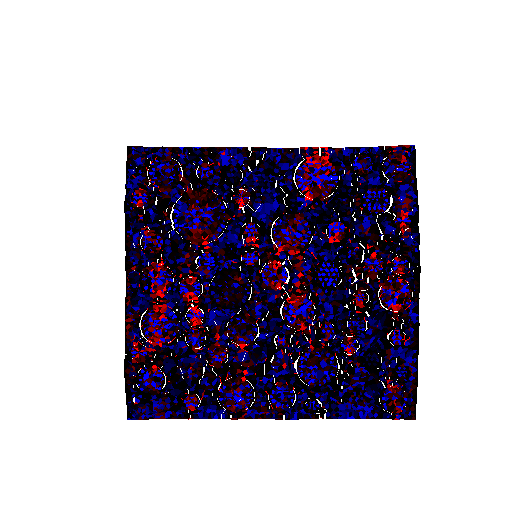
\includegraphics[width=1.0\linewidth]{Files/A30P75_3_IS_Free/DEP50-STEP(040).png}
      \caption{Loading Step 20}
      \end{subfigure}%
      %*******
      \begin{subfigure}{.33\textwidth}
        \centering
        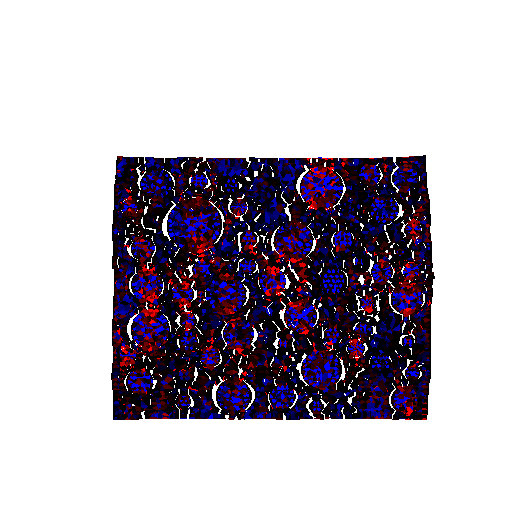
\includegraphics[width=1.0\linewidth]{Files/A30P75_3_IS_Free/DEP50-STEP(060).png}
        \caption{Loading Step 40}
      \end{subfigure}
      %*******

    %*******
    \begin{subfigure}{.33\textwidth}
      \centering
      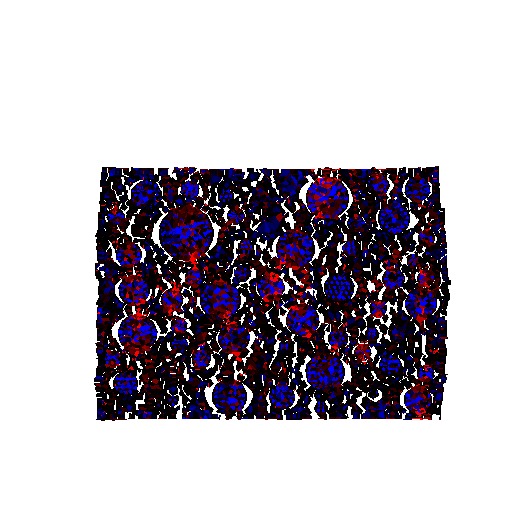
\includegraphics[width=1.0\linewidth]{Files/A30P75_3_IS_Free/DEP50-STEP(080).png}
      \caption{Loading Step 60}
    \end{subfigure}%
    \begin{subfigure}{.33\textwidth}
      \centering
      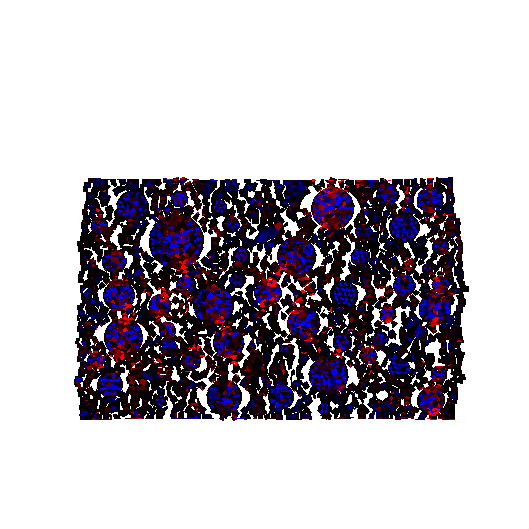
\includegraphics[width=1.0\linewidth]{Files/A30P75_3_IS_Free/DEP50-STEP(100).png}
      \caption{Loading Step 80}
      \end{subfigure}%
      %*******
      \begin{subfigure}{.33\textwidth}
        \centering
        \includegraphics[width=1.0\linewidth]{Files/A30P75_3_IS_Free/DEP50-STEP(120).png}
        \caption{Loading Step 100}
      \end{subfigure}
      %*******

      \begin{subfigure}{0.8\textwidth}
  \includegraphics[width=0.8\linewidth]{Files/exp_3D/tagCS30.png}
\end{subfigure}%


  \caption{ASR Loading in Free Boundary Condition}
  \label{fig:ASR_Loading_free}
\end{figure}


As for the displacement change in each step, Compressive Strength is also recorded to show the residual mechanical properties of the expanded model. Besides, Elastic Modulus will also be calculated from the plotting of the load-displacement graph.

\clearpage
\subsection{Experimental Result of ASR Expansion on Mechanical Properties of Concrete}

% [Swamy & Al-Asali, 1988]
In first test study, Swamy and Asali observed ASR-affected concrete in views of compressive strength, using 3 types Mixes (Control, 41/2\% opal, 15\% fused silica) for 1 year, in a cubic shape of size 100x100x100mm. The expansion is measured one-dimensionally.

The results found are in Figure \ref{Swamy1} as follow [Swamy \& Al-Asali, 1988].

\begin{figure}[h!]
  \centering
  \includegraphics[width=0.8\linewidth]{Reference/temp3.png}
  \caption{Effects of ASR expansion on compressive strength of concrete [Swamy \& Al-Asali, 1988].}
  \label{Swamy1}
\end{figure}


The compressive strength of opal concrete was 54\% less than that the control concrete for 28 days, then reached to 63\% at 1 year compared with the strength of control concrete. The loss in strength of fused silica concrete was nearly 26\% at 28 days and 39\% at 1 year as comparing it with that of control concrete [Swamy \& Al-Asali, 1988].

In Figure \ref{Swamy, Al-Asali, 1988 2}, the loss in compressive strength of control concrete and ASR-affected concrete at different rates of expansion was shown, where drop of compressive strength of ASR-affected concretes becomes more clear with expansion [Swamy \& Al-Asali, 1988].

\begin{figure}[h!]
\centering
%*******
\begin{subfigure}{.8\textwidth}
  \centering
  \includegraphics[width=1.0\linewidth]{Reference/temp5.png}
\end{subfigure}
%*******
\begin{subfigure}{.8\textwidth}
  \centering
  \includegraphics[width=1.0\linewidth]{Reference/temp6.png}
\end{subfigure}
%*******
\caption{Loss of compressive strength of ASR-affected concrete with time [Swamy \& Al-Asali, 1988]}
\label{Swamy, Al-Asali, 1988 2}
\end{figure}

\clearpage
%[Ahmed et al., 2003]
T. Ahmed et al. used Thames Valley sand (in Mix A), fused silica (in Mix B) and slowly reactive aggregate (in Mix C) to investigate the effect of ASR expansion on compressive strength of concrete, using specimens in size of 100x100x100 mm[BSEN 1290-3, 2000], cast and cured with respect to BS 1881 Part 122 [BS, 1881].

In this experiment, the cube specimens were cured for 28 days in water at 20$^\circ$C nd then the temperature was increased to 38$^\circ$C to accelerate alkali-silica reaction. Then specimens were stored at water tank until 12 months passed [Ahmed et al., 2003]. After 28-days curing at 20$^\circ$C and storage at 38$^\circ$C for 12 months, the expansion ratios and compressive strength are given in Figure \ref{Ahmed et al., 2003 1} [Ahmed et al., 2003].

% TODO: Remake Figure

\begin{figure}[h!]
  \centering
  \includegraphics[width=0.8\linewidth]{Reference/temp1.png}
  \caption{Effect of ASR expansion on compressive strength of concrete [Ahmed et al., 2003].}
  \label{Ahmed et al., 2003 1}
\end{figure}

As seen in Figure \ref{Ahmed et al., 2003 1}, the results reveal that compressive strength of Mix A is nearly 7.5\% higher than Mix C's (control mix) at 28 days due to no expansion in Mix A, while compressive strength of Mix A is nearly 12.7\% less than Mix C's (control mix) at 12 months due to its greater expansion compared with expansion of Mix C. As for Mix B, which is with fused silica, the greatest expansion in the three mixes is achieved and compressive strength dropped nearly 12.4\% for 28 days with compared to Mix C. After stored at hot water (38$^\circ$C) for 12 months, the drop in strength of Mix B reached to nearly 59.4\% [Ahmed et al., 2003].

%TODO: CHECK This
%As an another views, Cope and Slade observed an compressive strength increase in same mix (Mix A) and claimed that the curing of concrete including slowly reactive aggregate at high temperature doesn't affect overly on compressive strength of concrete at an early age or even after plenty time passes so compressive strength of Mix A can increase at 38$^\circ$C at this time [Cope & Slade, 1992].

Figure 3.1 reveals that a greater decrease in compressive strength was observed in Mix B compared with Mix A at any expansion percent due to different reaction rates for fused silia and Thames Vally sand permitting the hydration of cement to increase the compressive strength of concrete [Ahmed et al., 2003].

\begin{figure}[h!]
  \centering
  \includegraphics[width=0.8\linewidth]{Reference/temp2.png}
  \caption{Change in compressive strength of ASR-affected concrete vs. time [Ahmed et al., 2003].}
  \label{Ahmed et al., 2003 2}
\end{figure}

\clearpage
%[Smaoui et al., 2005]

Smaoui et al. carried out a study with some mechanical tests on the same topic by separating the specimens into 2 groups as Low-alkali concrete and High-alkali concrete. According to the test results, when the alkali content increased, a significant loss in the compressive strength of concrete appeared. As seen in Figure \ref{Smaoui et al., 2005 1}, the sharp loss in compressive strength of high-alkali concrete compared with low-alkali concrete's was initially shown at 3 days and then the rate of decline in strength loss changed slightly until 180 days pass. Moreover, the test results indicated that both of these concretes gained strength in 180-days test periods since the concretes were stored in the curing room at 23 0C and 100\% RH (Figure 3.4) [Smaoui et al., 2005]

\begin{figure}
  \centering
  \includegraphics[width=0.8\linewidth]{Reference/temp7.png}
  \caption{Difference in compressive strength between low-alkali concrete and high-alkali concrete [Smaoui et al., 2005]}
  \label{Smaoui et al., 2005 1}
\end{figure}

\clearpage
% GIANNINI(2012)

Giannini carried out mechanical properties test on expanded specimens damaged by ASR and DEF expansion. Two sets of 4 x 8 in. (100 x 200 mm) cylinders were produced for the purpose of further evaluating the effects of ASR and DEF on the mechanical properties of concrete. This study expands on and complements the mechanical tests conducted on the core samples extracted from the exposure site specimens. Two reactive aggregates, Jobe (F1) sand and Placitas (C10) gravel were used, bringing the total number of reactive aggregates investigated in the overall project to four. A non-linear resonant frequency test method was also employed for selected test specimens. In this study, the cylinders are intended to represent a laboratory analog for core samples extracted from a field structure.

Here the experiment results for ASR expansion are presented. Figure \ref{Giannini, 2012} shows the compressive strength results for the Jobe (F1) andPlacitas (C10) cylinders, respectively. Each data represents the average of three cylinders.

For the Jobe (F1) cylinders, decreases of 15\% were measured. For the Placitas (C10) cylinders, an increase of 17\% was measured for the ASR cylinders. The Placitas (C10) ASR cylinders expanded much more slowly than all other specimens in this study, and therefore were able to gain strength (possibly due to continued hydration of cement) more quickly than ASR could degrade it. However, the strength at 0.177\% expansion (approximately 8 months of age) was almost 18\% lower than that of the non-reactive control specimens at one year, so ASR did still have a negative impact on strength.

\begin{figure}[h!]
  \centering
  \includegraphics[width=0.8\linewidth]{Reference/GIANNINIASR.png}
  \caption{Elastic modulus and compressive strength results for ASR cylinders[Giannini, 2012]}
  \label{Giannini, 2012}
\end{figure}

\clearpage
%TODO: ALKANA(2013)

In study done by ALKANA (2014), the effect of ASR expansion on mechanical properties of concrete and the effect of specimen types on ASR expansion were investigated. Mechanical tests were performed on both the specimens exceeding expansion from ASR of 0.04 percent and ones exceeding that of 0.10 percent.

In this part, the results for G-A concrete with greater than expansion of 0.04 percent, G-B concrete with greater than that of 0.10 percent, and G-C concrete (control concrete) were given with graphs and tables in the following parts. While ASR-affected concrete (G-A, G-B) were started to be stored at 60$^\circ$C and 100\% RH, G-B concrete was compulsorily exposed to NaOH solution in recent weeks in order to provide expansion percentage of G-B concrete to exceed the limit of 0.10 percent. G-C concrete, on the other hand, was cured in water at 20$^\circ$C and used as control concrete. As known, the formed ASR gel absorbs water, expands, and causes internal pressure that causes cracking, which then continues and leads to expansion in concrete structure.



The ASR effect on compressive strength was examined by using cubic specimens, 150x150 mm in size, and cylindrical specimens, 100x200 mm in size. While the mix design of all specimens was prepared according to regulations as described by RILEM TC 219-ACS, compressive test for all specimens were carried out in accordance with the provisions in TS EN 12390-3. Limestone, non-reactive aggregate, and natural river sand, moderately reactive aggregate, were used as coarse and fine aggregates, respectively.

The expansion results in compressive strength for all specimens are given Figure \ref{ALKANA1}, Figure \ref{ALKANA2} and Figure \ref{ALKANA3}.

\begin{figure}[h!]
  \centering
  \includegraphics[width=1.0\linewidth]{Reference/ALKANASR1.png}
  \caption{Expansion and compressive strength of all concretes for cube specimens[ALKANA, 2012]}
  \label{ALKANA1}
\end{figure}

\begin{figure}[h!]
  \centering
  \includegraphics[width=1.0\linewidth]{Reference/ALKANASR2.png}
  \caption{Expansion and compressive strength of all concretes for cylindrical specimens[ALKANA, 2012]}
  \label{ALKANA2}
\end{figure}

\begin{figure}[h!]
  \centering
  \includegraphics[width=1.0\linewidth]{Reference/ALKANASR3.png}
  \caption{Loss in compressive strength of ASR-affected concrete comparing with control concrete [ALKANA, 2012]}
  \label{ALKANA3}
\end{figure}

\clearpage
\subsection{Summary of Experimental Result of ASR Expansion on Mechanical Properties of Concrete}

\begin{figure}[h!]
  \centering
  \includegraphics[width=1.0\linewidth]{Reference/GIANNINIASRdata.png}
\end{figure}

\begin{figure}[h!]
  \centering
  \includegraphics[width=1.0\linewidth]{Reference/ALKANASRdata.png}
\end{figure}

\begin{figure}[h!]
  \centering
  \includegraphics[width=1.0\linewidth]{Reference/AhmedASRdata.png}
\end{figure}

\begin{figure}[h!]
  \centering
  \includegraphics[width=1.0\linewidth]{Reference/SwamyASRdata_1.png}
\end{figure}

\begin{figure}[h!]
  \centering
  \includegraphics[width=1.0\linewidth]{Reference/SwamyASRdata_2.png}
\end{figure}


\clearpage
\subsection{Experimental Result of DEF Expansion on Mechanical Properties of Concrete}

% Bruetaud et al., 2008
In first test study, Bruetaud et al observed DEF-affected concrete in views of compressive strength. Figure \ref{Bruetaud Mix designs} summarizes the mix designs of these different concretes.

\begin{figure}[h!]
  \centering
  \includegraphics[width=0.8\linewidth]{Reference/Bruetaud1.png}
  \caption{Mix designs of the concrete, DEF cylinders[Bruetaud et al., 2008]}
  \label{Bruetaud Mix designs}
\end{figure}

Each concrete sample was cast and cured in 3 cylindrical moulds whose dimensions are 11 cm (diameter) and 22 cm (height) to generate 3 identical concrete specimens. The moulds were covered so as to limit water exchange. The applied heat treatment followed a cycle divided into four different steps, as shown in Figure \ref{Bruetaud heat}. Some concrete samples were not heat treated but were conventionally cured at 20 $^\circ$C to be used as reference. After the heat treatment, samples were stored at 20 $^\circ$C in 100\% relative humidity until 28 days. Next, wetting and drying cycles were applied in accordance with LPC no. 59 pre-test method, to increase the kinetics of DEF reaction without changing its triggering conditions. Samples are subjected to 2 cycles, each one lasting 14 days. A cycle consists of 7 days of drying at 38 $^\circ$C and 30\% relative humidity followed by 7 days of immersion in tap water at 20 $^\circ$C. The volume of water with respect to the volume of the sample is kept under 1.5 to limit leaching effects. Once the cycles are finished, samples are stored into 3 individual hermetic boxes (to avoid carbonation) whose dimensions barely exceed those of the sample, to minimize the amount ofwater required for their immersion.[Bruetaud et al., 2008]

\begin{figure}[h!]
  \centering
  \includegraphics[width=0.8\linewidth]{Reference/Bruetaud2.png}
  \caption{Heat treatment phases of DEF cylinders[Bruetaud et al., 2008]}
  \label{Bruetaud heat}
\end{figure}

During this last period, expansion measurements were performed with an extensometer whose resulting measurement dispersion on the basis of three concrete specimens is less than 0.002\%.

In the case of 0.48-Si concretes (“heating” experiments), a relationship can be obtained between the ultimate compressive strength (residual strength) and the final expansion achieved. Typically, the strength of unaffected 0.48-Si concrete specimens reaches about 40 MPa. The most damaged specimens of 0.48-Si concretes fall down to 15 MPa, which represents a very significant decrease.[Bruetaud et al., 2008]

In Figure \ref{Bruetaud CS}, the linear approximation would forecast a fall of strength on the order of 90\% for a 1.6\% expansion. This value, certainly exaggerated by the linear approximation, serves to verify that high expansion (over 1\%) leads to very low residual mechanical strength. The linear approximation proposed in Figure \ref{Bruetaud CS} seems to imply that a DEF-related expansion lower
than 0.20\% will not generate significant loss in compressive strength.[Bruetaud et al., 2008]

\begin{figure}[h!]
  \centering
  \includegraphics[width=0.8\linewidth]{Reference/Bruetaud3.png}
  \caption{Compressive stress versus final expansion for the concrete specimens of the
heating design of experiments[Bruetaud et al., 2008]}
  \label{Bruetaud CS}
\end{figure}

\clearpage
% GIANNINI(2012)

Together with ASR expansion, Giannini also carried out mechanical properties test on expanded specimens damaged by DEF expansion.

Similar two sets of 4 x 8 in. (100 x 200 mm) cylinders were produced for the purpose of further evaluating the mechanical properties of damaged concrete. Two types of aggregates, Jobe (F1) sand and Placitas (C10) gravel were used. A non-linear resonant frequency test method was also employed for selected test specimens. The cylinders are intended to represent a laboratory analog for core samples extracted from a field structure.

Here the experiment results for DEF expansion are presented. Figure \ref{Giannini, 2012 DEF} shows the compressive strength results for the Jobe (F1) andPlacitas (C10) cylinders, respectively. Each data represents the average of three cylinders. For the Jobe (F1) cylinders, decreases of 41\% were measured. For the Placitas (C10) cylinders, a decreas of 24\% is measured.[Giannini, 2012]

\begin{figure}[h!]
  \centering
  \includegraphics[width=0.8\linewidth]{Reference/GIANNINIDEF.png}
  \caption{Elastic modulus and compressive strength results for DEF cylinders[Giannini, 2012]}
  \label{Giannini, 2012 DEF}
\end{figure}

\clearpage
% Bouzabata et al., (2012)

In experiments performed by Bouzabata et al., DEF expansion for restrained and stress free on mortar prisms (40x40x160 mm) were presented. The water/cement ratio was 0.55 and the sand/cement ratio was 3. The chemical composition of the Portland cement used is given in Figure \ref{Bouzabata (2012)1}. As in the previous experiments, 3.1\% of $Na_2SO_4$ was added to the mixing water. Siliceous sand known to be non-alkali-reactive was used.

\begin{figure}[h!]
  \centering
  \includegraphics[width=0.8\linewidth]{Reference/Bouzabata1.png}
  \caption{Chemical compositions of cement and aggregate (\%) mortar prisms [Bouzabata et al., 2012]}
  \label{Bouzabata (2012)1}
\end{figure}

After casting, some of the specimens were cured at high temperatures with the heat treatment: 1 h at 20 $^\circ$C, an increase from 20 to 80 $^\circ$C in 4 h, a constant temperature of 80 $^\circ$C for 10 h then a cooling to 20 $^\circ$C in 10 h. The specimens were steamed in metal moulds, wrapped in watertight plastic film and covered by a metal plate to prevent evaporation of water during the heat treatment. At the same time, other specimens made in the same batch were stored at 20 $^\circ$C. After cooling and demoulding, specimens were kept at 20 $^\circ$C in endogenous conditions (sealed in plastic bags) for 28 days. [Bouzabata et al., (2012)]

Strains of specimens kept immersed in water after 28 days in stress-free conditions have been plotted in Figure \ref{Bouzabata (2012)2}. The specimens that had been subjected to the heat treatment during the curing period showed large expansions of between 1.3 and 2.2\% due to DEF. All the specimens in stress-free conditions exhibited mapcracking. The first significant cracks appeared for a strain of about 0.5\% (after 80 days of immersion in water). Compressive strength was measured on prismatic specimens (40x40x40mm) at time-steps chosen according to the expansions measured on the specimens (Figure \ref{Bouzabata (2012)2}).[Bouzabata et al., (2012)]

\begin{figure}[h!]
  \centering
  \includegraphics[width=0.8\linewidth]{Reference/Bouzabata2.png}
  \caption{Strain of specimens in stress-free conditions (each line corresponds to one specimen, specimens of a same batch are plotted with the same marker — dotted lines show the times of the mechanical tests). [Bouzabata et al., (2012)]}
  \label{Bouzabata (2012)2}
\end{figure}

The evolution of the compressive strength of the reference mortar and of the mortar damaged by delayed ettringite formation have been plotted in Figure \ref{Bouzabata (2012)3}. The reference specimens showed the usual increase of compressive strength with time due to continuous cement hydration. The specimens that had been subjected to the heat treatment showed a decrease in strength around 40\%. A large strength decrease occurred mainly between 70 and 100 days, corresponding to the significant increase of expansion, and the compressive strength reached a minimum value of 25MPa at 180 days.[Bouzabata et al., (2012)]

\begin{figure}[h!]
  \centering
  \includegraphics[width=0.8\linewidth]{Reference/Bouzabata3.png}
  \caption{Decrease of compressive strength according to DEF expansion [Bouzabata et al., 2012]}
  \label{Bouzabata (2012)3}
\end{figure}


\clearpage
% M. Al Shamaa et al., 2014

Figure 2 summarizes the mix design of the concrete used in the construction of the raft foundation. Concrete is made with calcareous
aggregates (in order to avoid the risk of alkali-aggregate reaction) and Portland cement CEM II/A-LL 42.5 R, which can be susceptible to an expansive behavior due to DEF. Concrete specimens were prepared according to the standards NF P 18-400 and NF P 18-422. Samples were cast in cylindrical molds whose dimensions are 11 cm (diameter) and 22 cm (height).

After casting, a part of concrete specimens was cured under heat treatments, shown in Figure \ref{Shamaa1}. The maximum temperature in cycle reached maximum 70$^\circ$C to expose concrete to a more severe condition by taking into account the variability of the properties of the material. Then the duration of the heat treatment was 18 days.

\begin{figure}[h!]
  \centering
  \includegraphics[width=0.8\linewidth]{Reference/Shamaa1.png}
  \caption{Experimental applied heat treatments [M. Al Shamaa et al., 2014]}
  \label{Shamaa1}
\end{figure}

Figure \ref{Shamaa_2} shows a comparison of compressive strength and Young’s modulus at the age of 28 days for different concretes.

\begin{figure}[h!]
  \centering
  \includegraphics[width=0.8\linewidth]{Reference/Shamaa2.png}
  \caption{Effect of heat treatment on the compressive strength and Young’s modulus
at 28 days. [M. Al Shamaa et al., 2014]}
  \label{Shamaa_2}
\end{figure}

Due to heat treatments, a decrease appeared of approximately 20\% of the compressive strength. This decrease was observed in both concretes T70-Im and T66-Im. Thus, the application of heat curing induces a lower value of mechanical resistance before the concrete is affected by DEF.

However, the Young’s modulus does not seem to be affected by the heat treatment. On the other hand, Figure \ref{Shamaa_3} shows that the concrete T70-Im, which suffers from DEF, presents a degradation of its mechanical properties. We observe a 23\% reduction in the compressive strength when the expansion was evolved from 0.08\% at the age of 180 days to 0.20\% at the age of 390 days. This loss is also observed for the Young’s modulus and may be an indicator of the damage of the material.

\begin{figure}[h!]
  \centering
  \includegraphics[width=0.8\linewidth]{Reference/Shamaa3.png}
  \caption{Relationship between the compressive strength, the Young’s modulus and
the expansion for concrete T70-Im. [M. Al Shamaa et al., 2014]}
  \label{Shamaa_3}
\end{figure}

However, the strength loss is not proportional to the expansion reached. In fact, we observe, according to our last measurements (at the age of 640 days when the expansion reaches 0.27\%), that the concrete tends to regain a part of its mechanical performance he had lost. This delayed re-increase is observed both on the compressive strength, the dynamic and the Young’s modulus.

These quantities have a minimum. Minima are observed at around 400 days when the inflection point of the slowdown in the expansion curve is reached Figure \ref{Shamaa_4}. On the other hand, all measurements on the concrete T66-Im concern only small expansions and the mechanical performances of this concrete was not affected until now (Figure \ref{Shamaa_5}).

\begin{figure}[h!]
  \centering
  \includegraphics[width=0.8\linewidth]{Reference/Shamaa4.png}
  \caption{Mechanical properties versus time for concrete T70-Im. [M. Al Shamaa et al., 2014]}
  \label{Shamaa_4}
\end{figure}

\begin{figure}[h!]
  \centering
  \includegraphics[width=0.8\linewidth]{Reference/Shamaa5.png}
  \caption{Relationship between the compressive strength, the Young’s modulus and
the expansion for concrete T66-Im. [M. Al Shamaa et al., 2014]}
  \label{Shamaa_4}
\end{figure}

\clearpage
\subsection{Summary of Experimental Result of DEF Expansion on Mechanical Properties of Concrete}

\begin{figure}[h!]
  \centering
  \includegraphics[width=1.0\linewidth]{Reference/GIANNINIDEFdata.png}
\end{figure}

\begin{figure}[h!]
  \centering
  \includegraphics[width=1.0\linewidth]{Reference/BruetaudDEFdata.png}
\end{figure}

\begin{figure}[h!]
  \centering
  \includegraphics[width=1.0\linewidth]{Reference/BouzabataDEFdata.png}
\end{figure}

\begin{figure}[h!]
  \centering
  \includegraphics[width=1.0\linewidth]{Reference/ShamaaDEFdata.png}
\end{figure}



%*******10********20********30********40********50********60********70********80
\clearpage

\section{Residual Capabilities after Pure ASR Expansion}

Here the uni-axial compression test result for ASR expanded concrete model is summarised.

\begin{figure}[ht]
\centering
\includegraphics[width=.3\linewidth]{Files/Aggregate/A30P75.png}
  \caption{30\% Coarse Aggregate}
  \label{fig:A30P75_model}
\end{figure}


%A30P75FIX

\begin{figure}[ht]
\centering
\includegraphics[width=.8\linewidth]{Files/exp_3D/ASR/S13A30P75FIX-LOAD-DISPLACEMENT.png}
  \caption{A30 P75 Fix Load-Displacement}
  \label{fig:A30P75FIX_LD}
\end{figure}




%A30P75FREE

\begin{figure}[ht!]
\centering
\includegraphics[width=.8\linewidth]{Files/exp_3D/ASR/S13A30P75FREE-LOAD-DISPLACEMENT.png}
  \caption{A30 P75 Free Load-Displacement}
  \label{fig:A30P75FREE_LD}
\end{figure}

\begin{table}[ht!]
\centering
\begin{tabular}{ ||p{2cm}|p{2cm}|p{2cm}|p{3cm}|p{3cm}|| }
 \hline
  Initial Strain (Each Step) & Expanding Steps & Final Expansion [\%] & Maximum Compressive Strength in Fix Loading Condition [MPa] & Maximum Compressive Strength in Free Loading Condition [MPa]\\ [0.5ex]
 \hline\hline
  0 & 0 & 0 & 29.987 & 19.897\\
  0.0002 & 20 & 0.0699 & 27.601 & 13.889\\
  0.0005 & 20 & 0.1936 & 25.339 & 9.8203\\
  0.001 & 20 & 0.4223 & 22.667 & 7.4466\\
  0.002 & 20 & 0.8832 & 18.725 & 5.8732 \\
  0.003 & 20 & 1.3224 & 15.993 &\\

 \hline
\end{tabular}
\caption{One Dimensional Expansion Ratio in Single ASR Model Simulation}
\label{table:ASR_30_EXP}
\end{table}

From the Figure \ref{fig:A30P75FIX_LD} and Figure \ref{fig:A30P75FREE_LD} it can be seen that with the increasing of given initial strain in each step, its global expansion ratio also increasing, and both maximum compressive strength in fix boundary condition and free boundary condition gradually decrease.




%A30P25FIX
\begin{figure}[ht]
\centering
\includegraphics[width=.3\linewidth]{Files/Aggregate/A30P25.png}
  \caption{30\% Coarse Aggregate}
  \label{fig:A30P25_model}
\end{figure}

\begin{figure}[ht]
\centering
\includegraphics[width=.8\linewidth]{Files/exp_3D/ASR/S13A30P25FIX-LOAD-DISPLACEMENT.png}
  \caption{A30 P25 Fix Load-Displacement}
  \label{fig:A30P25FIX_LD}
\end{figure}

%A15P75FIX

\begin{figure}[ht]
\centering
\includegraphics[width=.3\linewidth]{Files/Aggregate/A15.png}
  \caption{15\% Coarse Aggregate}
  \label{fig:A15P75_model}
\end{figure}

\begin{figure}[ht]
\centering
\includegraphics[width=.8\linewidth]{Files/exp_3D/ASR/S13A15P75FIX-LOAD-DISPLACEMENT.png}
  \caption{A15 P75 Fix Load-Displacement}
  \label{fig:A15P75FIX_LD}
\end{figure}


%*******10********20********30********40********50********60********70********80
\clearpage

\section{Residual Capabilities after Pure DEF Expansion}

%A30X0FIX

\begin{figure}[ht]
\centering
\includegraphics[width=.8\linewidth]{Files/exp_3D/DEF/S13A30FIXX0-LOAD-DISPLACEMENT.png}
  \caption{A30 I50 Fix Load-Displacement}
  \label{fig:A30X0FIX_LD}
\end{figure}

%A30X-5FIX

\begin{figure}[ht]
\centering
\includegraphics[width=.8\linewidth]{Files/exp_3D/DEF/S13A30FIXX-5-LOAD-DISPLACEMENT.png}
  \caption{A30 I75 Fix Load-Displacement}
  \label{fig:A30X-5FIX_LD}
\end{figure}

%A30X-1FIX

\begin{figure}[ht]
\centering
\includegraphics[width=.8\linewidth]{Files/exp_3D/DEF/S13A30FIXX-1-LOAD-DISPLACEMENT.png}
  \caption{A15 I50 Fix Load-Displacement}
  \label{fig:A30X-1FIX_LD}
\end{figure}

%A15X0FIX

\begin{figure}[ht]
\centering
\includegraphics[width=.8\linewidth]{Files/exp_3D/DEF/S13A15FIXX0-LOAD-DISPLACEMENT.png}
  \caption{A15 I50 Fix Load-Displacement}
  \label{fig:A15X0FIX_LD}
\end{figure}


%*******10********20********30********40********50********60********70********80
\clearpage

\subsection{Result And Discussion}

In this section, the relationship between concrete's behavior of expansion and its losses on mechanical properties are discussed.

By RBSM, all information of the 3-dimensional cracking behavior can be recorded and analysis numerically. While it is with difficulties to summarized the behavior of expansion by the naked eye, all stress distribution and crack generation process are able to be analyzed numerically.

For example, in Figure \ref{fig:Total_Number_of_Cracks}, the relationship of total cracked interfaces and its relationship with residual compressive strength (in a ratio of the compressive strength of undamaged model) is presented.

It can be seen that as the total cracking interfaces number increase, the residual compressive strength decrease in all kinds of expansion applied.

\begin{figure}[ht!]
\centering
\includegraphics[width=.8\linewidth]{Files/exp_3D/Residual_Compressive_Strength_vs_Total_Number_of_Cracks.png}
  \caption{Residual Compressive Strength vs. Total Number of Cracks}
  \label{fig:Total_Number_of_Cracks}
\end{figure}

While structually, larger crack in width do represent larger damage, especially in its mechanical properties, here in Figure \ref{fig:Total_Number_of_Cracks_0.0005+} the relationship between total number of cracked interfaces larger than 0.0005 mm and the residual compressive strength is plotted.

This time clear linear relationship between the number of cracks larger than 0.0005 mm and the reducing in its compressive strength can be seen here, both in ASR expansion and DEF expansion.

\begin{figure}[ht!]
\centering
\includegraphics[width=.8\linewidth]{Files/exp_3D/Residual_Compressive_Strength_vs_Total_Number_of_0005_Cracks.png}
  \caption{Residual Compressive Strength vs. Total Number of Cracks over 0.0005 mm}
  \label{fig:Total_Number_of_Cracks_0.0005+}
\end{figure}

If plot the total number of cracked interfaces larger than 0.001 mm and the residual compressive strength, as shown in Figure \ref{fig:Total_Number_of_Cracks_0.001+}, similar trand is shown, indicate that the number of wider cracks largely determined the residual compressively strength.
\begin{figure}[ht!]
\centering
\includegraphics[width=.8\linewidth]{Files/exp_3D/Residual_Compressive_Strength_vs_Total_Number_of_001_Cracks.png}
  \caption{Residual Compressive Strength vs. Total Number of Cracks over 0.001 mm}
  \label{fig:Total_Number_of_Cracks_0.001+}
\end{figure}

While if plotting the total number of cracked interfaces relately smaller and the residual compressive strength, the linear corrisbonding relationship does not show up, and shown in Figure \ref{fig:c1}, Figure \ref{fig:c2}, and Figure \ref{fig:c3}. This result indicte that the residual compressive strength is less depends on smaller scale cracks comparing to the larger cracks.

\begin{figure}[ht!]
\centering
\includegraphics[width=.8\linewidth]{Files/exp_3D/1.png}
  \caption{Residual Compressive Strength vs. Total Number of 0.0005+mm Cracks}
  \label{fig:c1}
\end{figure}

\begin{figure}[ht!]
\centering
\includegraphics[width=.8\linewidth]{Files/exp_3D/2.png}
  \caption{Residual Compressive Strength vs. Total Number of 0.001+mm Cracks}
  \label{fig:c2}
\end{figure}

\begin{figure}[ht!]
\centering
\includegraphics[width=.8\linewidth]{Files/exp_3D/3.png}
  \caption{Residual Compressive Strength vs. Total Number of 0.002+mm Cracks}
  \label{fig:c3}
\end{figure}


This result implied that while the expansion mechanism and cracking pattern can be different in ASR and DEF expansion, the residual mechanical properties, for example, the compressive strength, is determined by the existence of larger cracks (0.005 mm+ here). This may offer us a new direction in the analysis the residual capacity of the expanded concrete structure.

The relationship found here also explained the reason of differences in loss of mechanical properties when same global scale expansion applied by different mechanisms. As the cracking pattern caused by ASR and DEF are different, shown in Figure \ref{fig:expcs}, their mechanical properties loss in same expansion can be different.

At same one-dimensional global expansion, shown in Figure \ref{fig:ASR_A30P75_3_3Dsss} and Table \ref{table:ASRs_30_EXP}, ASR expanded models have more larger cracks, while cracks causes by DEF are relately concentrated in smaller width range. As the result, in our simulation, ASR have less residual compressive strength comparing to DEF cases.

\begin{figure}[ht!]
\centering
\includegraphics[width=.8\linewidth]{Files/exp_3D/EXPvsCS.png}
  \caption{Residual Compressive Strength vs. Expansion[\%]}
  \label{fig:expcs}
\end{figure}


\begin{figure}[ht!]
\centering
    %*******
    \begin{subfigure}{.33\textwidth}
      \centering
      \includegraphics[width=.8\linewidth]{Files/exp_3D/ASR/A30P75_3_3d.png}
    \end{subfigure}%
    %*******
    \begin{subfigure}{.33\textwidth}
      \centering
      \includegraphics[width=.8\linewidth]{Files/exp_3D/DEF/A30X0C_3_3d.png}
    \end{subfigure}%
    %*******
    \begin{subfigure}{.33\textwidth}
      \centering
      \includegraphics[width=.8\linewidth]{Files/exp_3D/DEF/A30X-5C_3_3d.png}
    \end{subfigure}
    %*******
    %*******
    \begin{subfigure}{.33\textwidth}
      \centering
      \includegraphics[width=.8\linewidth]{Files/exp_3D/ASR/A30P75_3_3ds.png}
      \caption{ASR A30 P75 Case 3 \\ Surface Crack}
    \end{subfigure}%
    %*******
    \begin{subfigure}{.33\textwidth}
      \centering
      \includegraphics[width=.8\linewidth]{Files/exp_3D/DEF/A30X0C_3_3ds.png}
      \caption{DEF A30 I50 Case 3 \\ Surface Crack}
    \end{subfigure}%
    %*******
    \begin{subfigure}{.33\textwidth}
      \centering
      \includegraphics[width=.8\linewidth]{Files/exp_3D/DEF/A30X-5C_3_3ds.png}
      \caption{DEF A30 I75 Case 3 \\ Surface Crack}
    \end{subfigure}
    %*******
    %*******
    \begin{subfigure}{.33\textwidth}
      \centering
      \includegraphics[width=0.8\linewidth]{Files/exp_3D/ASR/A30P75_3_c.png}
      \caption{ASR A30 P75 Case 3 \\ Internal Stress}
    \end{subfigure}%
    %*******
    \begin{subfigure}{.33\textwidth}
      \centering
      \includegraphics[width=0.8\linewidth]{Files/exp_3D/DEF/A30X0C_3_c.png}
      \caption{DEF A30 I50 Case 3 \\ Internal Stress}
    \end{subfigure}%
    %*******
    \begin{subfigure}{.33\textwidth}
      \centering
      \includegraphics[width=0.8\linewidth]{Files/exp_3D/DEF/A30X-5C_3_c.png}
      \caption{DEF A30 I75 Case 3 \\ Internal Stress}
    \end{subfigure}
    %*******
    %*******
    \begin{subfigure}{.33\textwidth}
      \centering
      \includegraphics[width=1.0\linewidth]{Files/exp_3D/ASR/A30P75_3_stress.png}
      \caption{ASR A30 P75 Case 3 \\ Internal Stress}
    \end{subfigure}%
    %*******
    \begin{subfigure}{.33\textwidth}
      \centering
      \includegraphics[width=1.0\linewidth]{Files/exp_3D/DEF/A30X0C_3_stress.png}
      \caption{DEF A30 I50 Case 3 \\ Internal Stress}
    \end{subfigure}%
    %*******
    \begin{subfigure}{.33\textwidth}
      \centering
      \includegraphics[width=1.0\linewidth]{Files/exp_3D/DEF/A30X-5C_3_stress.png}
      \caption{DEF A30 I75 Case 3 \\ Internal Stress}
    \end{subfigure}
    %*******
  \caption{Cracking Pattern Compare}
  \label{fig:ASR_A30P75_3_3Dsss}
\end{figure}

\begin{table}[ht!]
  \caption{One Dimensional Expansion Ratio in Single ASR Model Simulation}
\centering
\begin{tabular}{ |p{4cm}|p{2cm}|p{3cm}|p{3cm}| }
 \hline
 Case &  Final Expansion  & Number of cracked face over 0.0005 mm & Residual Compressive Strength\\ [0.5ex]
 \hline
 ASR A30P75 Case 3 & 0.4223 & 357498 & 0.7559 \\ \hline
 DEF A30I50 Case 3 & 0.5795 & 379069 & 0.7835 \\ \hline
 ASR A30I75 Case 3 & 0.5118 & 332827 & 0.7931 \\
 \hline
\end{tabular}

\label{table:ASRs_30_EXP}
\end{table}

\section{Conclusion}

In this chapter, three-dimensional expanded concrete models are tested under uni-axial compression condition, and the mechanical properties obtained from simulation are compared with previous experimental results from other researchers.

Details about the residual mechanical properties, including residual compressive strength and residual elastic modulus in each loading case for ASR and DEF expansion, are summarized.

The relationships between residual capacity and expansion behavior due to different expansion causes are also discussed.

Linear relationship between the number of cracks larger than 0.0005 mm and the reducing in its compressive strength can be seen both in ASR expansion and DEF expansion, implied that while the expansion mechanism and cracking pattern can be different in ASR and DEF expansion, the residual mechanical properties, for example, the compressive strength, is determined by the existence of larger cracks.

Though relationship between cracking and compressive strength is obtained in this research, the relationship with elastic modulus is still unclear. For our simulation result in elastic modulus is significantly lower than experimental result, adjustment in material properties may required in further research.

